\ifx\allfiles\undefined
\documentclass{XDBAthesis}
\def\pictures{}
\begin{document}
\else
\fi
\chapter{Demo实现与测试结果}
前文我们详细介绍了我们提出的手机拍照手势识别算法,并从理论上分析了其可行性。本章我们将在实际情况下完成一个Android平台的Demo,并进行测试,给出测试结果。
\section{测试环境}
测试手机为:魅族MX2
编译环境为:Mac OS X 10.10.3,1.7GHz Intel Core i7,8GB 1600MHz DDR3,128G SSD。
所有代码均利用Android Studio 1.2,Java在JRE 1.6.0,C++在Clang 600.0.56环境下编译完成。
\section{Demo框架}

\section{软件运行结果展示}
我们利用本算法开发了个简单拍照demo,其主要功能是检测手动作,并进行相应操作:上划放大,下划缩小,左划倒计时3s拍照,右划倒计时5s拍照。
\subsection{手势识别在OpenCV上的实现}
图\ref{fg:1}为算法后台运行的log。可见,我们的算法采用间接抓取的方式,以16FPS的频率抓取图片,并处理展示。当识别到相应手势时现在log中显示,再进行相应操作。
\begin{figure}[htb]
    \centering
    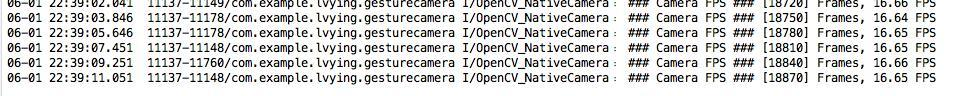
\includegraphics[width=0.5\textwidth ]{figure/opencvframe}%
    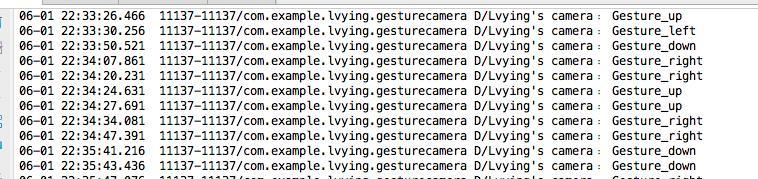
\includegraphics[width=0.5\textwidth ]{figure/gesture}
    \caption{log记录}
    \label{fg:1}
\end{figure}
\subsection{CPU与系统内存占用}
CPU与系统内存占用如图\ref{fg:2}所示。可见,本算法对内存及计算量的要求并不算高,可以实际运用。
\begin{figure}[htb]
    \centering
    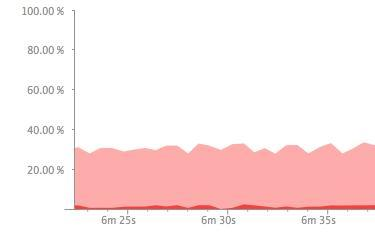
\includegraphics[width=0.5\textwidth ]{figure/cpu}%
    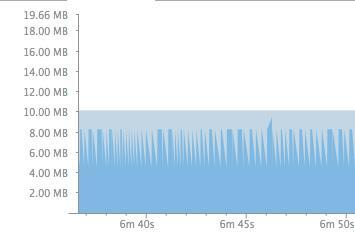
\includegraphics[width=0.5\textwidth ]{figure/memory}
    \caption{CPU与内存消耗占比图}
    \label{fg:2}
\end{figure}
\subsection{手势捕捉与处理}
当手势被识别后,进行对应功能处理。如果进入拍照功能,在屏幕右上角显示倒计时3秒,并在倒计时结束时拍照。如果是放大或缩小功能,由于前置摄像头无法实现物理变焦,故采用数字放大/缩小实现该功能。因为识别为动态过程,不方便截图展示,因此我们只截取了一个识别到左划手势并开始拍照倒计时的界面,和一个拍照完成的提示。如图\ref{fg:3}所示。
\begin{figure}[htb]
    \centering
    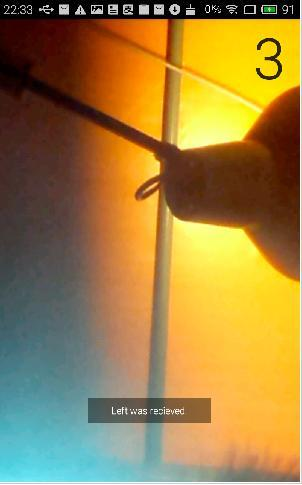
\includegraphics[width=0.3\textwidth ]{figure/recognize}%
    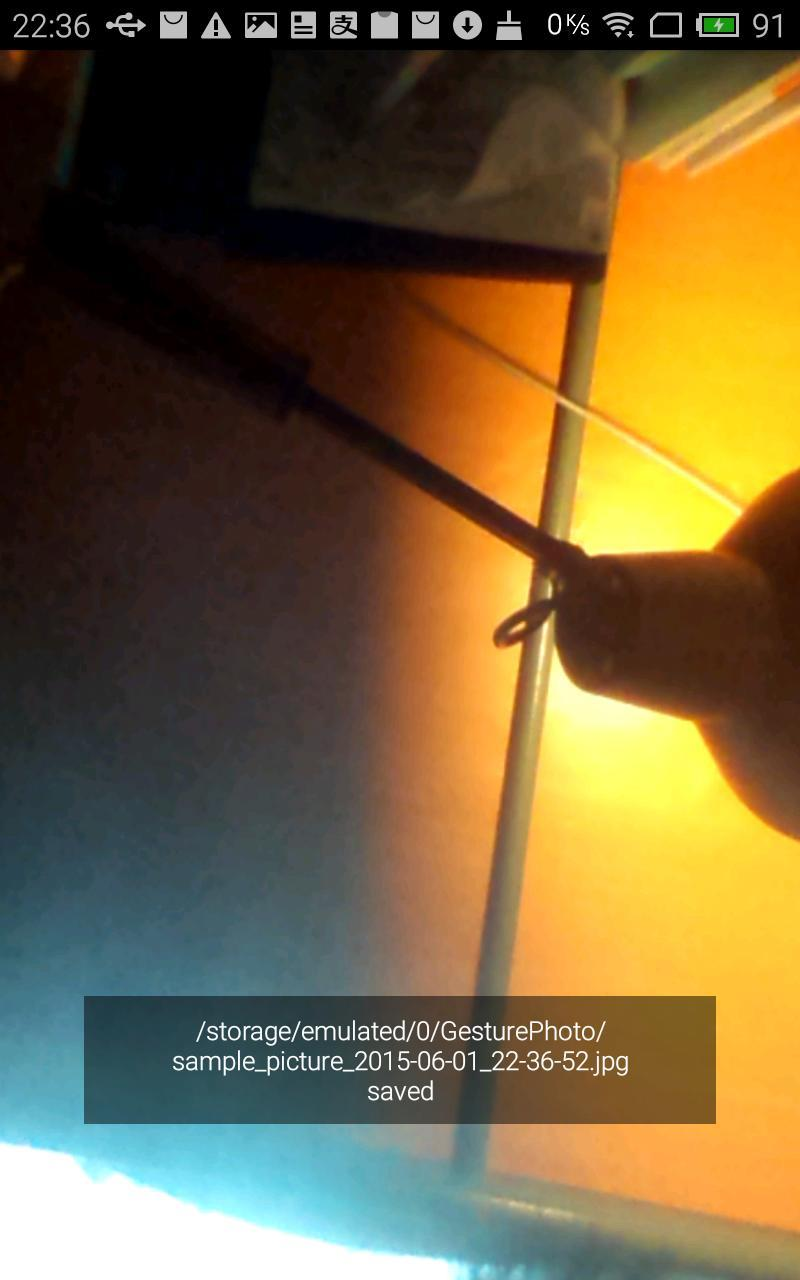
\includegraphics[width=0.3\textwidth ]{figure/capture}
    \caption{手势识别演示}
    \label{fg:3}
\end{figure}

%经过实验,我们可知在准确度,速度,稳定性上本算法均以达到实用标准。本算法已具有实际使用的可行性。

\ifx\allfiles\undefined
%\bibliographystyle{unsrt}
\bibliography{main}
\end{document}
\fi